\documentclass[twocolumn,twoside]{IEEEtran}
\usepackage[hidelinks]{hyperref}
\usepackage{graphicx}
\usepackage{float}
 \usepackage{epstopdf}
\usepackage{changepage}
\usepackage{pbox}
\usepackage{tabularx}
\usepackage[official]{eurosym}

\def\sectionautorefname{Section}
\def\figureautorefname{Figure}

\def\BibTeX{{\rm B\kern-.05em{\sc i\kern-.025em b}\kern-.08em
    T\kern-.1667em\lower.7ex\hbox{E}\kern-.125emX}}

\newtheorem{theorem}{Theorem}
\setcounter{page}{1}

\begin{document}

\title{CloudSicle: A Cloud Implementation of Gifsicle}

\author{\IEEEauthorblockN{Christiaan Titos Bol\'{i}var (\href{mailto:C.TitosBolivar@student.tudelft.nl}{C.TitosBolivar@student.tudelft.nl}),  
Quinten Stokkink (\href{mailto:Q.A.Stokkink@student.tudelft.nl}{Q.A.Stokkink@student.tudelft.nl})
\thanks{C.Titos Bol\'{i}var and Q. Stokkink are students of the Computer Science department of the Delft
University of Technology (TUDelft)}}
\phantom{Hello :D}
\\\IEEEauthorblockA{\textit{Course Instructors}
: Alexandru Iosup and Dick Epema PDS Group, EEMCS ([\href{mailto:A.Iosup@tudelft.nl}{A.Iosup},\href{mailto:D.H.J.Epem@tudelft.nl}{D.H.J.Epema}]@tudelft.nl)}
\IEEEauthorblockA{\textit{Lab Assistant}
: Bogdan Ghit PDS Group, EEMCS (\href{mailto:B.I.Ghit@tudelft.nll}{B.I.Ghit@tudelft.nl})}
}

\markboth{IN4392: Cloud Computing}
{Titos Bol\'{i}var and Stokkink: CloudSicle}

\maketitle
%\thispagestyle{plain}\pagestyle{plain}

\begin{abstract}
This article explains how to use a \LaTeX\ class that produces a good
approximation to the style used in the IEEE Transactions.  The article
is itself an example of the IEEEtran.cls class in action.
\end{abstract}

\section{Introduction}
\label{sec:intro}
\PARstart{S}{ince} the dawn of the internet people have sought to 
enrich their internet experience. As we have gone from plain 
text to richt text to eventually images accompanying text, in 1987 we 
eventually ended up with the Graphics Interchange Format or \textit{.gif} which
made its way onto our webpages.

We have seen databases work their way onto the internet to communicate
data to users (e.g. SQL) and we have seen Cloud storage systems to communicate files
over the internet (e.g. Facebook, Google Drive, etc.). In other words, we have seen
these developments which are the respective counterparts of delivering
textual content on a large scale and delivering images on a large scale.
Following the history of the internet, the obvious next step would then be
delivering \textit{.gif}s on a large scale. This is where CloudSicle comes into play.

CloudSicle is an application we developed as a proof of concept to 
check the feasibility of Cloud Computing to deliver a rich internet experience.
The goal of the application is to process multiple images into one (animated) image in a large scale context. For the sake of implementation
we have focused ourselves on the communication between a client,
a server and allocated Virtual Machines instead of trying to integrate this all into a 
webpage context. Furthermore, as our scope lies with the scalability
and speed of the Virtual Machine processing, we have outsourced the
creation of the actual \textit{.gif}s to an application called \textit{Gifsicle}\cite{gifsicle}.
\textit{Gifsicle} is a free and open source command-line tool created
by Eddie Kohler for the creation of animated \textit{.gif}s.

In the end we hope to present \textbf{WantCloud BV} with an implementation
design and concept, which can be used to provide a \textit{.gif}
creation service to other businesses. The need of the future.

The structure of this report will be as follows:
\begin{itemize}
\item In \autoref{sec:require} we will lay out our requirements.
\item \autoref{sec:design} will explain the design of CloudSicle as well as some implementation details.
\item We evaluate CloudSicle with a number of experiments shown in \autoref{sec:eval}
\item In \autoref{sec:eval} we will discuss the main findings of our work as well as the trade-offs of using CloudSicle.
\end{itemize}

\section{Requirements}
\label{sec:require}
In this section we will first provide some background information concerning CloudSicle. Following this we will list the requirements we have formulated  together with \textbf{WantCloud BV}.

Animated gifs are a popular internet phenomenon. These images usually are short in duration. Long animated gifs result in a large file size and thus a large loading time online. The duration of an animated gif often is no more than a 2 to 6 seconds. At a framerate of 24 fps we assume the average number of frames of an animated gif is about a 100. We therefore choose this as the average workload per request CloudSicle has to work with.

As mentioned in the previous section we designed CloudSicle 
for future deployment in a large setting. This means that CloudSicle
should scale very well according to usage. Apart from scaling up
we also define coping with varying levels of usage as scaling down
in a timely fashion as well. Scaling down can improve resource utilization and can reduce costs as well as we only pay for what we use.

Our second target was to have the system respond as fast as
possible. Creating animated gifs is fast, and thus the overhead of the cloud infrastructure should be kept to minimal. This means we would like to always serve requests as they come in. 

%We need to take into account that CloudSicle should calculate what the fastest path to completion
%is. For example, using one Virtual Machine to do all of the work
%may be several orders of magnitude faster than allocating three
%Virtual Machines and having two of them share partial results to
%the third machine which combines the results and sends them back.

%In theory we can calculate the point where the overhead of
%adding a new machine to the resource pool would be worth it 
%(using some greedy scheduling algorithm).
%However, in practice things like Virtual Machine start-up time
%and overall system pressure are hard, if not impossible, to 
%predict. This makes job end times variable and generally
%unknown (which are essential for scheduling algorithms). 
%Therefore, we use the experiments as will be laid
%out in \autoref{sec:eval} to come up with good heuristics for predicting
%when Virtual Machines should be added or removed.

The summarization of our requirements is therefore as follows:
\begin{LaTeXdescription}
\item[Automation] The system should handle the resource management autonomously. \hfill \
\item[Intelligent Scaling] The system should scale up under high pressure, and scale down under low pressure \hfill \
\item[Responsiveness] The response time and makespan should be kept minimal. \hfill \
\item[Job Allocation] Optimal job partitioning over VMs to ensure that VMs are not inactive during their entire lifespan.\hfill \
\item[Reliability] Failed jobs should be automatically restarted.\hfill \
\item[Monitoring] Administrators should be able to monitor the entire CloudSicle system.\hfill \
\end{LaTeXdescription}

\section{System Design}
\label{sec:design}
. In this section we will discuss the system 
design and interactions between these actors and how they apply
to the homonym features as requested by \textbf{WantCloud BV} 
(\textit{Automation}, \textit{Elasticity}, \textit{Performance}, \textit{Reliability}, \textit{Monitoring}). 
The visualization
of this behavior is depicted in \autoref{fig:systemdesign} for
reference. 

\begin{figure}[h]
\begin{center}
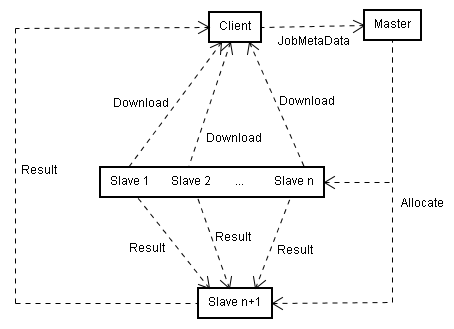
\includegraphics[width=88mm,keepaspectratio=true]{general_cloudsicle}
\caption{CloudSicle overall system design for some arbitrary Single Layer VM \textit{SplitJob} strategy}
\label{fig:systemdesign}
\end{center}
\end{figure}

\subsection{Architecture}
As previously mentioned the CloudSicle software consists of one or more clients, all of which connect to a server which can allocate Virtual Machines. We will reference the server as the \textit{Master} and the Virtual Machines that it creates as \textit{Slaves}, \textit{Slave VMs} or just \textit{VMs}. The Client, Master and Slaves communicate through structured messages. The application flow is started by a Client sending a request to the Master. This request contains a list of files (as well as data such as the number of files and the total file size) that the client wants to have combined. The Master maintains a job queue, in which all incoming requests are stored before they are scheduled. The Scheduler will select the request at the head of the queue and will then allocate one or more VMs from the Resource Pool to process this request according to some allocation policy. Once the Slave is done, it will send the resulting file back to the Client.

We define several types of messages that can be passed between Client, Master and Slaves.
\begin{LaTeXdescription}
\item[JobMetaData] The request made by the Client is packed in a JobMetaData message. These objects are used by the master to allocate VMs.
\item[Activity] An Activity consists of a number of \emph{Jobs} a Slave has to execute in a certain sequence. 
\item[StatusUpdate] A Slave will send updates about its status to the Master via StatusUpdate messages throughout the execution. For monitoring purposes this also includes the type of \emph{Job} currently being executed.
\end{LaTeXdescription}

As mentioned, an Activity message will consist of a list of jobs that the Slave must execute. These possible jobs are:
\subsubsection{DownloadJob}
The DownloadJob instructs the Slave to actively contact some other Slave or the Client and download a given set of files.
The Master will set up this situation beforehand, such that the offering party has the files offered for download when the
Slave attempts to download them.
\subsubsection{WaitForResultsJob}
 The second way to receive input files is using a passive mechanism with a WaitForResultsJob, where the Slave waits for all the input files to be sent over by
other Slaves before undertaking action. This is also the only time a Slave will every have to wait before executing its jobs.
\subsubsection{CombineJob}
The CombineJob will process the downloaded input files with \emph{Gifsicle} and stream the output to the Slave's disk.
\subsubsection{CompressJob}
The result of the CombineJob might be further processed by compressing it into a so-called \textit{Tarball}. This is done before the result is sent back to the Client to minimize the network pressure of sending data on the outbound line of the data center. The Master can issue this compression using the CompressJob.
\subsubsection{ForwardJob}
The last step for every Slave VM will be to forward its result, which may be output in the form of a \textit{.gif} file or a \textit{.tar.gz} file (depending on the Activity), and send it to the next Slave or a Client.
For the Slave itself it does not matter who will download its result. After performing the delivery to some other party all of the input files and result(s) are removed from its file system and the Slave will either \emph{(a)} signal the Master that it is done with its Activity, marking it as available for the next Activity or \emph{(b)} shut itself down if it has been marked
by the Master to exit on Acitivy completion (\emph{SoftExit}).

If any of the Jobs of an Activity fail, the Master will shutdown the VM and reschedule the entire JobMetaData request by putting it at the end of the job queue.
This ensures system reliability.

\subsection{Resource Management}
One of the most important requirements is the scaling of the resource pool of VMs. If there are few requests, we only need a single VM, if there are many, then perhaps we need more.

The Master maintains a Resource Pool consisting of Slave VMs. The pool has three lists; an \emph{AvailableVMs} list, containing all the VMs that are booted and are waiting for a Job, a \emph{VMsInUse} list containing all the VMs that are currently executing an Activity, and an \emph{allVMs} list containing all the VMs that have been used throughout the lifetime of the Master (this list is for monitoring purposes). Each Slave VM can execute one Activity at a time.

We already mentioned the short nature of the jobs that CloudSicle requests have. When requests are sparse, the overhead of creating a new VM every time would be too large. We therefore make sure we always have one running VM instance in our resource pool. If a request arrives while all VMs are busy, we create a new VM. The scheduler will then wait until a VM becomes available. This could be a busy VM that has finished in the meantime, or the newly created VM that has finished booting. When a VM is done with its Activity it will added back to \emph{AvailableVMs} list. 

To ensure scaling down, after a VM is done with an Activity, the Master will wait a certain amount of time before shutting down the VM and removing it from the Resource Pool. Note that this only happens when a VM is done with an Activity. If it has yet to execute something, it will remain active. Because we always have at least one VM in the pool, and jobs are short, making the need for extra VMs low, the timeout can be very short. In  our proof of concept implementation, we set this time out to 6 seconds. In our experiments we show that this value yields good results.

\subsection{Job Allocation}
Requests are scheduled in a first come first serve manner. We have defined two allocation schemes for CloudSicle, \emph{SingleJob} and \emph{SplitJob}.
\subsubsection{SingleJob} 
\emph{SingleJob} is a straightforward allocation policy that will simply use one Slave to process the entire request. The Master will pass all the files of the JobMetaData to the DownloadJob of the Slave.
\subsubsection{SplitJob}
\emph{SplitJob} is a more sophisticated policy. Because it is possible to merge two animated gifs, we are able to divide the input files over multiple Slaves, produce partial results that will then be combined again by another Slave, resulting in an animated gif consisting of all the input files (this is the example shown in \autoref{fig:systemdesign}). 

The ForwardJob of the "intermediate" Slaves will pass the result to the Slave that is designated by the Master to produce the final results. This final Slave will use the WaitForResults job to wait until all other Slaves have sent their partial results. It will then combine and compress as usual and forward the final result to the Client.

This approach bears similarity to a MapReduce computation \cite{MapReduce}.
Depending on the strategy an arbitrary amount of distinct
layers can be introduced. This means CloudSicle can simulate
a MapReduce computation with two distinct mapping layers for
a given constant amount of iterations (N.B. constant, as the forwarding between
Slaves is defined beforehand).

Another strategy that could be simulated is an inverse
tree computation for additional speed at the cost of higher
overhead (\emph{log(n)} Virtual Machines instead of the constant
amount of Virtual Machines required by MapReduce). 

\subsection{System Policies}
\subsubsection{Overhead reduction}
To avoid Slaves wasting time polling during a WaitForResultsJob,
we can have Slaves invoke other Slaves to download files from them. 
This is done in an effort to shorten the time a Slave waits for its 
input files and to remove the CPU overhead of busy waiting.

To avoid the Master polling
the Slaves for status updates we make the Slaves
report their state changes to the Master. To further save on communication
cost we can also mark Slaves to exit once their current set of
jobs is finished. We can afford this autonomy of Slaves as the
jobs they execute are stateless in respect to the rest of the
system: if any of the jobs fail, the Slave fails as a whole and if
all jobs succeed, the Slave presents only the end result.

\subsubsection{Security}
The security policies for Cloudsicle are limited, but not completely
ignored. Communication between the Client and the Master
happens through SSH (Secure Shell). This offers some protection
from external intervention and limits the set of attackers to 
individuals authorized on the TUDelft VPN (Virtual Private Network). 
Any communication between the
Master and Slaves, as well as Slaves between each other is handled
inside the datacenter (using local IPs). 
Slaves sending their result back to the Client  
is done on a default Java SSL (Secure Socket Layer) connection,
but still with use of the VPN.
In the course of data mitigating over the CloudSicle system
this data is also never evaluated, only transformed.
As an added security measure all files are only passed on by
their file id handle (integer), with only output having a special
file id handle. This is a security weak point and might allow
external attackers to identify and alter data being sent to
Clients.

\subsection{Monitoring}
The Master has a Monitor service that keeps track of all the statuses of Slaves in the system (and logs them).
It stores JobMetaData for these Slaves and records changes in the Jobs that the Slaves
are currently executing (Executing \emph{DownloadJob}, executing \emph{CombineJob}, etc.). 
For Slaves it is recorded whether in what state they are, and the corresponding JobMetaData
is then stored in one of the following states:
\begin{LaTeXdescription}
\item[Waiting] The JobMetaData is awaiting allocation to a Slave
\item[Running] The jobs of the JobMetaData are being executed on a Slave
\item[Finished] All of the jobs of the JobMetaData have been successfully run.
\item[Failed] One of the jobs of the JobMetaData has failed.
\end{LaTeXdescription}
When the Monitor gets updated by the Master if a change in one of the Jobs happens,
it records the time of the event. This allows the Monitor to calculate the
average completion time of a set of jobs and the average amount of time spent
on each of the jobs.
We used the Monitor to get our experimental results (as will be presented in \autoref{sec:setup}).

\subsection{Implementation}
We have implemented a proof of concept of our design. It is written in Java, and can be found on Github\footnote{\url{https://github.com/ChrisTitos/CloudSicle}}.

The CloudSicle project distributes three runnable \emph{.jar} files.
These are \emph{client.jar}, \emph{master.jar} and \emph{slave.jar}.
It also requires a user to specify his log-in credentials in a \emph{config.txt},
here communication ports for normal messages and file transfers can also
be specified.

A client can run his software by placing his \emph{client.jar} and \emph{config.txt}
in the same folder and then run the \emph{client.jar}. The client will
be presented by a small interface that allows him to select files, the DAS4
server entry point and send his (automaticly inferred) JobMetaData to the master.
When the activity has been processed the resulting \emph{.tar.gz} compressed
folder will appear in the client's folder.

The master will be deployed by sending the \emph{master.jar}, the \emph{slave.jar}
and the \emph{config.txt} to the DAS4 server. The service is then started by
running the \emph{master.jar}. The \emph{slave.jar} is automaticly deployed to
any Slave VMs the master creates. To stop the service the administrator
can simply press the \emph{enter}-key to clean up all allocated Virtual Machines.
Should the application crash or be forefully terminated, the administrator will
have to shut down all the allocated Virtual Machines by hand.

\section{Experimental Results}
\label{sec:setup}
In this section we will lay out the setup of our tests
our rationale for testing things in this fashion and the
results of each test. Apart from the default metrics
we will also report the amount of files per hour increments and 
the cost if the Amazon EC2 rate of 10 Eurocents per
hour were used per file.

\subsection{Experimental setup}
Our system was deployed on the DAS-4 cluster\cite{das4}.
For Virtual Machine monitoring we made use of the 
Java OpenNebula Cloud API \cite{opennebulaapi}.
To avoid having our tools interfering with the process
we measured the makespans (in seconds), for differing
input sizes,
on the Master (using the Monitor, as discussed earlier) only using the standard Java system calls
for timing.
These different input sizes consisted of instances of
multiple of the same file being fed into the system, each exactly 54870 bytes in size. 
Due to complications in the implemenation phase, we were
only able to test the \emph{SingleJob} strategy: which is
arguably the least interesting strategy we support.

\subsection{Experiment 1: Makespans}
In the first experiment we measured the makespans of 
different activity sizes. We created datasets of different
sizes with the same file. The sizes we created are:
\begin{LaTeXdescription}
\item[Small] A set containing only 2 images
\item[Medium] A set containing 20 images
\item[Large] A set containing 100 images, which is our expected activity size
\item[Jumbo] A set containing 1000 images
\item[Immense] A set containing 6739 images, which is the maximum amount \emph{cp} would produce on our system
\end{LaTeXdescription}
\autoref{fig:makespans} depicts the running time in seconds 
for each of these datasets. For the medium and jumbo datasets
we have also given a more detailed insight into the specific
jobs that are executed in \autoref{fig:makespanexpl}.

An interesting observation to be made from \autoref{fig:makespans},
is that the time it takes per file to handle a job decreases from
6.5 seconds per file to 0.15 seconds per file (see \autoref{tab:makespans}). If we make a rough
inverse exponential approximation of this data we see that the algorithm
becomes 'efficient' (second order derivative is 0) at about 500 input files.

We can observe from \autoref{fig:makespanexpl} is that smaller jobs
are prodominantly defined by the time it takes to forward their
result, accounting for about 50\% of the job. As the job gets
bigger, we see that this shifts to the downloading taking up
most of the time of the job, taking again about 50\% of the job.
What we can also observe is that compression time takes up
a larger percentage of the job time as it gets bigger, waiting
time and combination time stay about the same and forward time shrinks percentually.

We expected the forward time and waiting time to be more or less constant
with regard to the input size. We see in \autoref{fig:makespanexpl} however,
that the waiting time grows with the input size. Upon further investigation
it appeared that this is caused due to the increased time the Client
needs to send his JobMetaData. The time JobMetaData spends in the waiting
queue is virtually the same.

\begin{figure}[h]
\begin{center}
 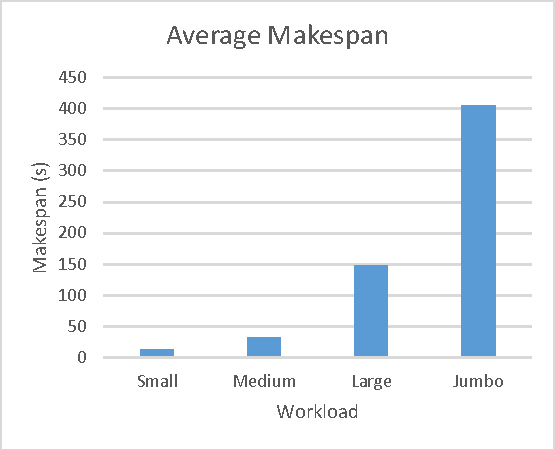
\includegraphics[trim=0 0 0 0,keepaspectratio=true,scale=0.8]{makespan}
\caption{The average makespan of a single job}
\label{fig:makespans}
\end{center}
\end{figure}

\begin{figure}[h]
\begin{center}
 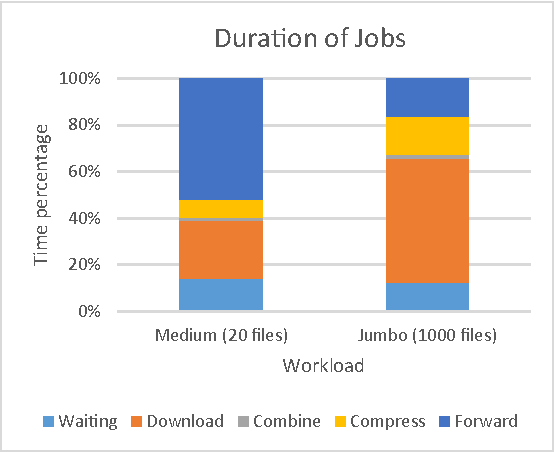
\includegraphics[trim=0 0 0 0,keepaspectratio=true,scale=0.8]{jobdurations}
\caption{The makespan of the medium and jumbo workload, average time spent per job type for the activity}
\label{fig:makespanexpl}
\end{center}
\end{figure}

\begin{table}[htb]
\caption{Single Slave per activity}
\label{tab:makespans}

\begin{center}

{\tt
\setlength{\tabcolsep}{.16667em}
\begin{tabularx}{92mm}{|l||X|X|X|X|X|}
\hline
Observed &Small&Medium&Large&Jumbo&Immense\\\hline\hline
files&2&20&100&1000&6739\\\hline
total size (MB)&0.1&1.1&5.5&54.8&369.8\\\hline
makespan (s)&13&33&148&405&1015\\\hline
\end{tabularx}
} 
\end{center}

\begin{center}

{\tt
\setlength{\tabcolsep}{.16667em}
\begin{tabularx}{92mm}{|l||X|X|X|X|X|}
\hline
Inferred &Small&Medium&Large&Jumbo&Immense\\\hline\hline
time per file (s)&6.5&1.65&1.48&0.40&0.15\\\hline
files / hour&554&2182&2432&9000&24000\\\hline
\pbox{2.5cm}{EC2 cost/file (10\textsuperscript{-4} EUR)}&1.80&0.45&0.41&0.11&0.04\\\hline
\end{tabularx}
}
\end{center}
\end{table}

\subsection{Experiment 2: Scaling}
One of the most important requirements of CloudSicle is the autoscaling of VM resources. To evaluate the autoscaling capabilities of CloudSicle we needed to simulate a semi realistic workload over a certain time span. We do this by generating 20 requests (of the medium workload) at random time intervals between 1 and 30 seconds.

\autoref{fig:scaling} shows the scaling of the resources over time. We see the total amount of VMs in the systems scales well with the number of jobs running. There is a nice buffer of available VMs, especially during periods where there are multiple VMs running at the same time. This would suggest that during consistent high request levels, CloudSicle will scale up accordingly. Scaling down is also shown in intervals 404 to 443. Another observation is the fact that jobs rarerely stay in the job queue of the Scheduler for more than a second.


\begin{figure*}[ht]
\begin{center}
\begin{adjustwidth}{}{}
  \resizebox{\textwidth}{!}{%
 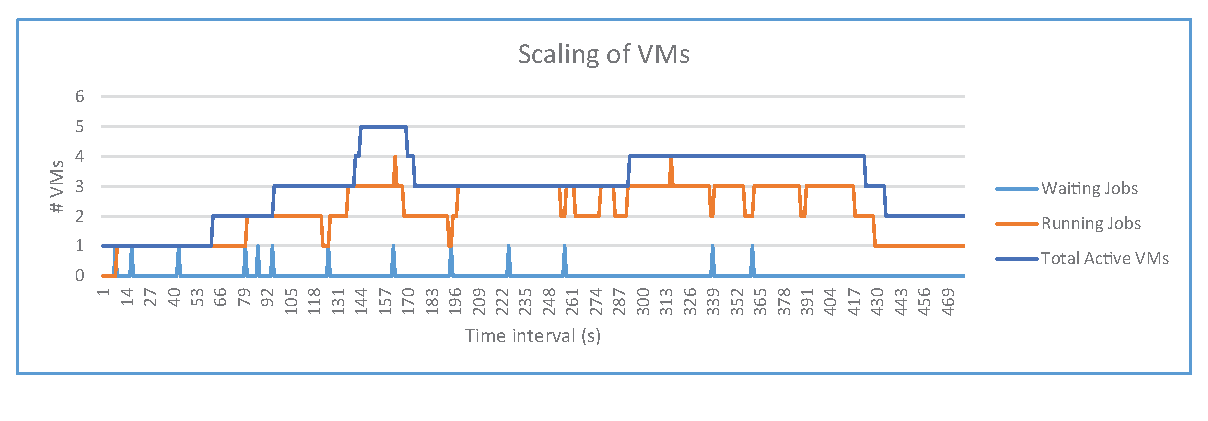
\includegraphics{scaling.eps}
} \end{adjustwidth}
\caption{The behaviour of CloudSicles resource scaling}
\label{fig:scaling}
\end{center}
\end{figure*}


\begin{table}
\caption{The created VMs during experiment 2. The utilization is calculated by multiplying the average running time of a request (59 s)  by the number of requests a VM has processed. Because we take the average request time, the utilization of VM \#39154 is too high.}
\begin{tabularx}{92mm}{|l||X|X|X|X|X|}
\hline 
VM ID & Running/ Charged Time & Requests Processed & Utilization & Costs \\
\hline 
\hline 
\#39159 & 199 & 2 & 59\% & \euro{0,10} \\
\hline 
\#39158 & 405 & 3 & 44\% &  \euro{0,10} \\
\hline 
\#39157 & 390 & 4 & 61\% & \euro{0,10} \\
\hline 
\#39156 & 482 & 3 & 37\% &  \euro{0,10} \\
\hline 
\#39155 & 255 & 1 & 23\%  &  \euro{0,10} \\
\hline 
\#39154 & 334 & 7 & 124\% &  \euro{0,10} \\
\hline 
\end{tabularx}
\end{table}


\begin{table}
\caption{Overview of VM usage metrics for Experiment 2}
\begin{tabularx}{92mm}{|l||X|X|}
\hline 
Total Running time:	& 2065 s \\
\hline 
Average running Time & 344 s \\
\hline 
Total requests processed: & 20 \\
\hline 
Average VM running time per job & 17,21 s \\
\hline 
Average utilization & 58\% \\
\hline 
Total cost & \euro{0,60} \\
\hline 
Cost per request & \euro{0,03} \\
\hline 
\end{tabularx}
\end{table}

\section{Evaluation}
\label{sec:eval}
In this section the evaluation of the experimental results as given in \autoref{sec:setup} will be discussed.
First the observed and inferred results of the two experiments we performed will be discussed.
The second half of this section will deal with the extrapolation of these results.

\subsection{Results}
%summarize the main findings of your work and discuss the tradeoffs inherent in the design of
%cloud-computing-based applications.Should the WantCloud CTO use IaaS-based clouds?

\subsection{Extrapolation}
%Among others, use extrapolation on the results, as reported in Section 6.b of the report, to discuss the charged time and
%charged cost reported in section for 100,000/1,000,000/10,000,000 users and for 1 day/1 month/1 year. 
As discussed in the introduction of this report, we assume the average CloudSicle job to contain 100 files on average.
Given the calculated cost per file from \autoref{tab:makespans} we can calculate the costs for 100 thousand, 1 million and 10 million users.
For these calculations we assume have set the maximum amount of Slaves to 20.
The result of these calculations is given in \autoref{tab:extracharge}, we note that because we have
not tested the splitting of jobs the increase with the amount of users is linear.

\begin{table}[htb]
\caption{Extrapolated Charge Time \& Cost}
\label{tab:extracharge}
\begin{center}
{\tt
\begin{tabular}{|c||c|c|}
\hline
Users (Millions)&Time (Hours)&Cost(EUR)\\\hline\hline
0.1&206&420\\\hline
1&2056&4120\\\hline
10&20556&41120\\\hline
\end{tabular}
} 
\end{center}
\end{table}

For all of the possible combinations of days, weeks, months and years in combination
with millions of users we can also calculate the cost. If we filter out the impossible
amounts of hours per timeframe we get the results of \autoref{tab:extracost}.
These calculation assume the worst case scenario where Virtual Machines get
all of their work at once and the rest of the time the buffer Virtual Machine
remains powered on. This causes maximum inefficiency in CloudSicle's buffering
scheme.

\begin{table}[htb]
\caption{Extrapolated Cost Per Day}
\label{tab:extracost}
\begin{center}
{\tt
\begin{tabular}{|c|c||c|}
\hline
Users (Millions)&Per&Cost(EUR)\\\hline\hline
0.1&Month&471\\\hline
0.1&Year&1254\\\hline
1&Year&4790\\\hline
\end{tabular}
} 
\end{center}
\end{table}

We note that the implementation of the SplitJob would drastically change the
outcome of these calculations. If Virtual Machines are able to balance loads and
continuously accept activities, the throughput of the system would be much
higher (and therefore the cost would be much lower).

\section{Conclusion}
\label{sec:concl}

\section*{Acknowledgments}
\noindent The authors would like to acknowledge the guidance of A. Iosup and
D. Epema in exploring the world of Cloud Computing and offering
the authors the chance to interact with the DAS-4 system.
The authors would also like to acknowledge B. Ghit for his interactions
when the authors were unable to log in to DAS-4 and also when OpenNebula
accounts were needed.

\begin{appendices}
\section{Time Sheet}
This section contains the times spent on various things while developing
and testing CloudSicle in \autoref{tab:timetot}. It also contains times per experiment 
(\autoref{tab:timee1} for experiment 1 and \autoref{tab:timee2} for experiment 2).
\begin{table}[htb]
\caption{Totaltime}
\label{tab:timetot}
\begin{center}
{\tt
\begin{tabular}{|c|c|}
\hline
Activity&Hours\\\hline\hline
total-time&141\\\hline
think-time&8\\\hline
dev-time&108\\\hline
xp-time&7\\\hline
analysis-time&4\\\hline
write-time&14\\\hline
wasted-time&0\\\hline
\end{tabular}
} 
\end{center}
\end{table}
\begin{table}[htb]
\caption{Experiment 1 Time}
\label{tab:timee1}
\begin{center}
{\tt
\begin{tabular}{|c|c|}
\hline
total-time&4.5\\\hline
dev-time&0.5\\\hline
setup-time&4\\\hline
\end{tabular}
} 
\end{center}
\end{table}
\begin{table}[htb]
\caption{Experiment 2 Time}
\label{tab:timee2}
\begin{center}
{\tt
\begin{tabular}{|c|c|}
\hline
total-time&2.5\\\hline
dev-time&0.5\\\hline
setup-time&2\\\hline
\end{tabular}
} 
\end{center}
\end{table}

\end{appendices}

\nocite{*}
\bibliographystyle{IEEE}
%%%%%\bibliography{bib-file}  % commented if *.bbl file included, as seen below

%%%%%%%%%%%%%%%%% BIBLIOGRAPHY IN THE LaTeX file !!!!! %%%%%%%%%%%%%%%%%%%%%%%%
%% This is nothing else than the IEEEsample.bbl file that you would          %%
%% obtain with BibTeX: you do not need to send around the *.bbl file         %%
%%---------------------------------------------------------------------------%%
%
\begin{thebibliography}{1}
\bibitem{gifsicle}
Kohler, E.
\newblock {\em Gifsicle: Command-Line Animated GIFs},
\newblock {\url{http://www.lcdf.org/gifsicle/}},
\newblock {Last retrieved October 30 2013}

\bibitem{MapReduce}
Dean, J., \& Ghemawat, S.  
\newblock {2008}.
\newblock {\em MapReduce: simplified data processing on large clusters}. 
\newblock {Communications of the ACM, 51(1), 107-113}.

\bibitem{das4}
University of Amsterdam
\newblock {\em DAS-4 Overview},
\newblock {\url{http://www.cs.vu.nl/das4/}},
\newblock {Last retrieved October 30 2013}

\bibitem{opennebulaapi}
Open Nebula
\newblock {\em Java OCA API 2.0},
\newblock {\url{http://opennebula.org/documentation:archives:rel2.0:java}},
\newblock {Last retrieved October 30 2013}

\end{thebibliography}
%
%%---------------------------------------------------------------------------%%


\end{document}

%%%%%%%%%%%%%%%%%%%%%%%%%%%  End of IEEEsample.tex  %%%%%%%%%%%%%%%%%%%%%%%%%%%


